\section{Components}
\begin{figure}
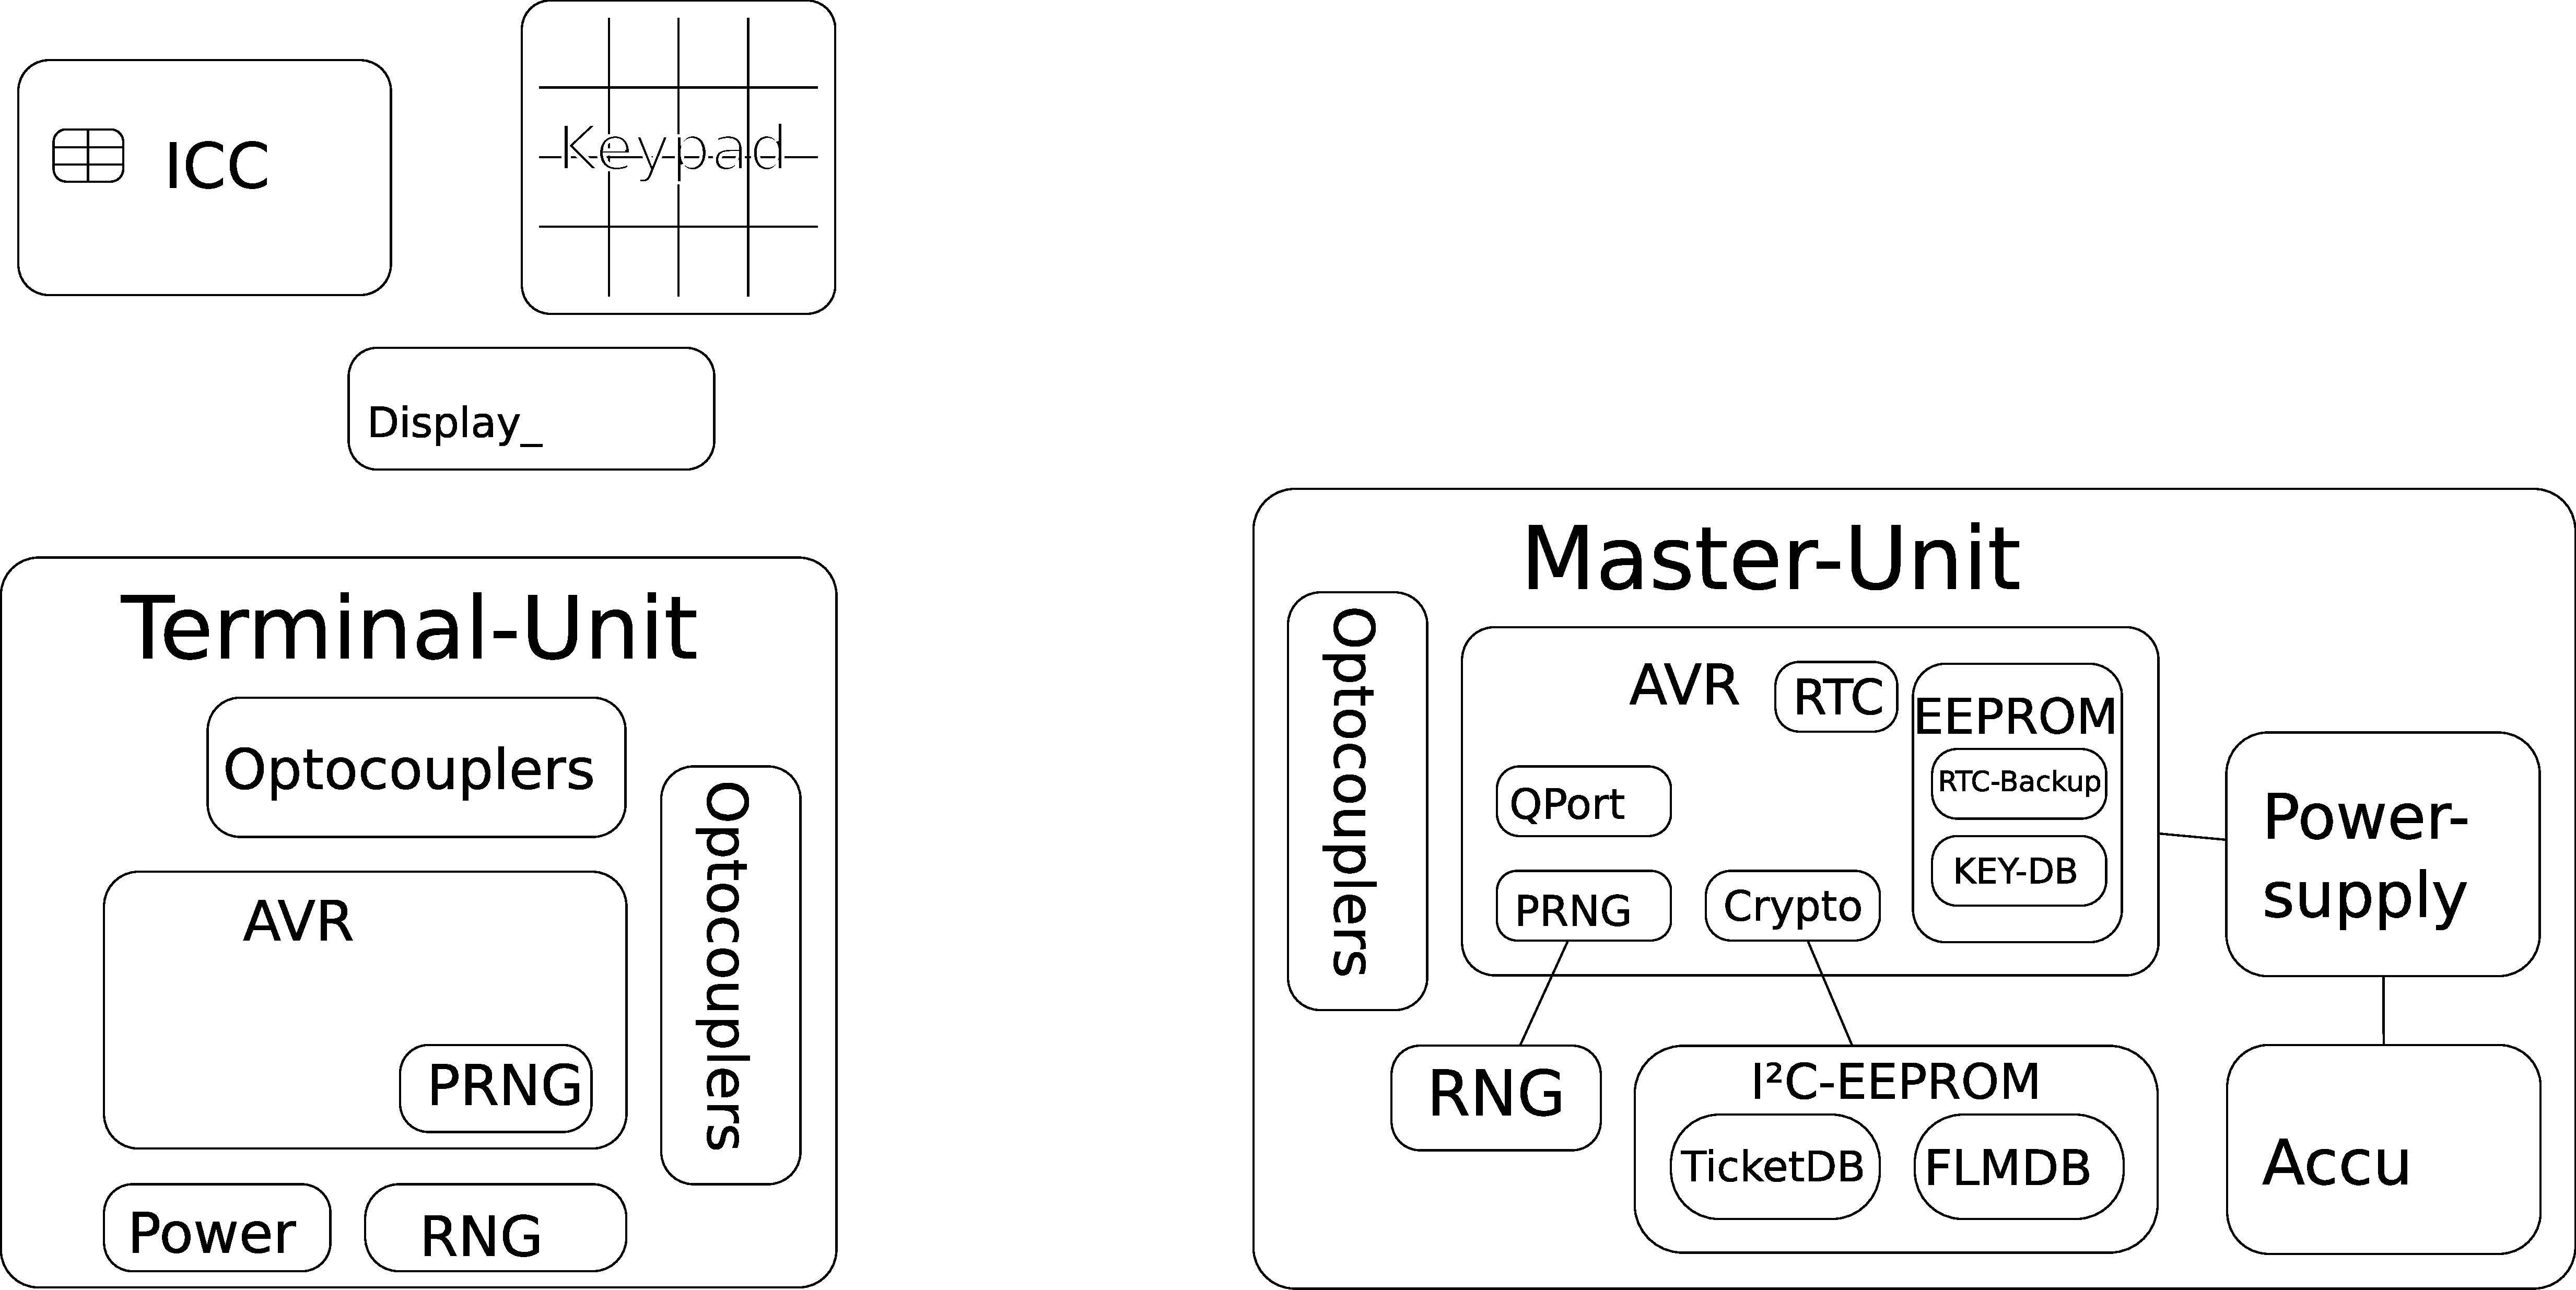
\includegraphics[scale=0.17]{Overview} 
\caption{system overview}
\end{figure}
The AnonAccess system is divided in \textit{Terminal-Unit} and \textit{Master-Unit} also there is a chipcard for each user which stores user's authentification data.

%-----

\subsection{Chip-Card}
We use simple memory cards with $I^2C$-Bus\cite{I2C} and form factor ID-1 as specified in \cite{ISO7816-1}\cite{ISO7816-2}. They are quite cheap (less then 1\euro{} per card) and not secure. Their contents might easily be read or modified. So everyone can read and check what we write on his/her card.

The card contains a so called \textit{AuthBlock} embedded in an ASN.1-BER\cite{ASN.1BER} octal-string object
The \textit{AuthBlock} has the following structure:\\
\begin{tabular}{|l|c|l|} \hline
name & size & description \\ \hline 
UID            & 2 bytes & index to the \textit{TicketDB} \\
ticket         & 32 bytes & ticket containing encrypted time-stamp \\
$r_{key}$ & 32 bytes & random key for $r_{ID}$ decryption \\
$r_{ID}$   & 32 bytes & encrypted user pseudonym \\
HMAC        & 32 bytes & $HMAC_{absign\_key}(UID \parallel ticket \parallel r_{key} \parallel r_{ID})$\\ \hline
\end{tabular} 

%-----

\subsection{Terminal-Unit}
The \textit{Terminal-Unit} handels userinputs, displays information and reads and writes the user's card.
It is equipted with keypad, display, cardreader and a hardware random number generator. It is powered by the \textit{Master-Unit} and should therefore not be reseted even in the case of power failure.
%-----

\subsection{Master-Unit}
The \textit{Master-Unit} keeps the databases, does the authentication and executes the managed the secured action (ex. opens a door).
%-----

\subsection{Power supply}

%-----

\subsection{Real time clock (RTC)}
The real time clock is implemented in software by using one of the microcontroller's timers. A timer interrupt function increments a 64bit value each millisecond (this counter will wrap around in about 584.542.046 years, which should be quite enough for us). Additionally the counter's value is periodically\footnote{the value is backed up every $3FFFFF_{(16)}$ milliseconds which is about every 1.165 hours} written to the microcontroller's EEPROM and read back after reset. On reset we also add the value $3FFFFF_{(16)}$ to the counter to avoid having the same timestamp, for more than one time.

The backup storage is implemented in a ring buffer structure with an additional index byte. 
The index byte indicates which cell of the ring buffer is to be used. After writing a value to a cell it is read back and checked. If the check fails the index byte is incremented by one and the next cell is used. The EEPROM is specified to be written 100,000 times so one cell may work for 116,508.4 hours which is about 13.29 years. So with a ring buffer of 20 cells, we should be able to operate for about 265.82 years which should be sufficient for most applications (if not the ring buffer could be easily made even larger).

It should be known that the timer value does not necessarily correspond to a linear continous timeline or human time, although the time is monotonic increasing. % extend me
%-----

\subsection{Microcontroller}
We use microcontrollers from the ATmega family from Atmel\cite{Atmel}for both units. They are relatively cheap and support protection of the internal memories (flash and EEPROM) from being read by their lock-bit feature. There also is a toolchain including GCCs\cite{GCC} C-compiler and a libc implementation\cite{AVR-Libc} available for these 8 bit microcontrollers which eases the writing of the software.

The \textit{Master-Unit} uses an ATmega644\cite{ATmega644} in DIL-Package with 64KiB of program flash, 4KiB of internal SRAM and 2KiB of internal EEPROM (100,000 rewrite cycles guaranteed).

The \textit{Terminal-Unit} uses an ATmega32\cite{ATmega32} in DIL-Package with 32KiB of program flash, 2KiB of internal SRAM and 1KiB of internal EEPROM (100,000 rewrite cycles guaranteed).
 
%-----

\subsection{Random number generator (RNG)}
\begin{window}[0,r, 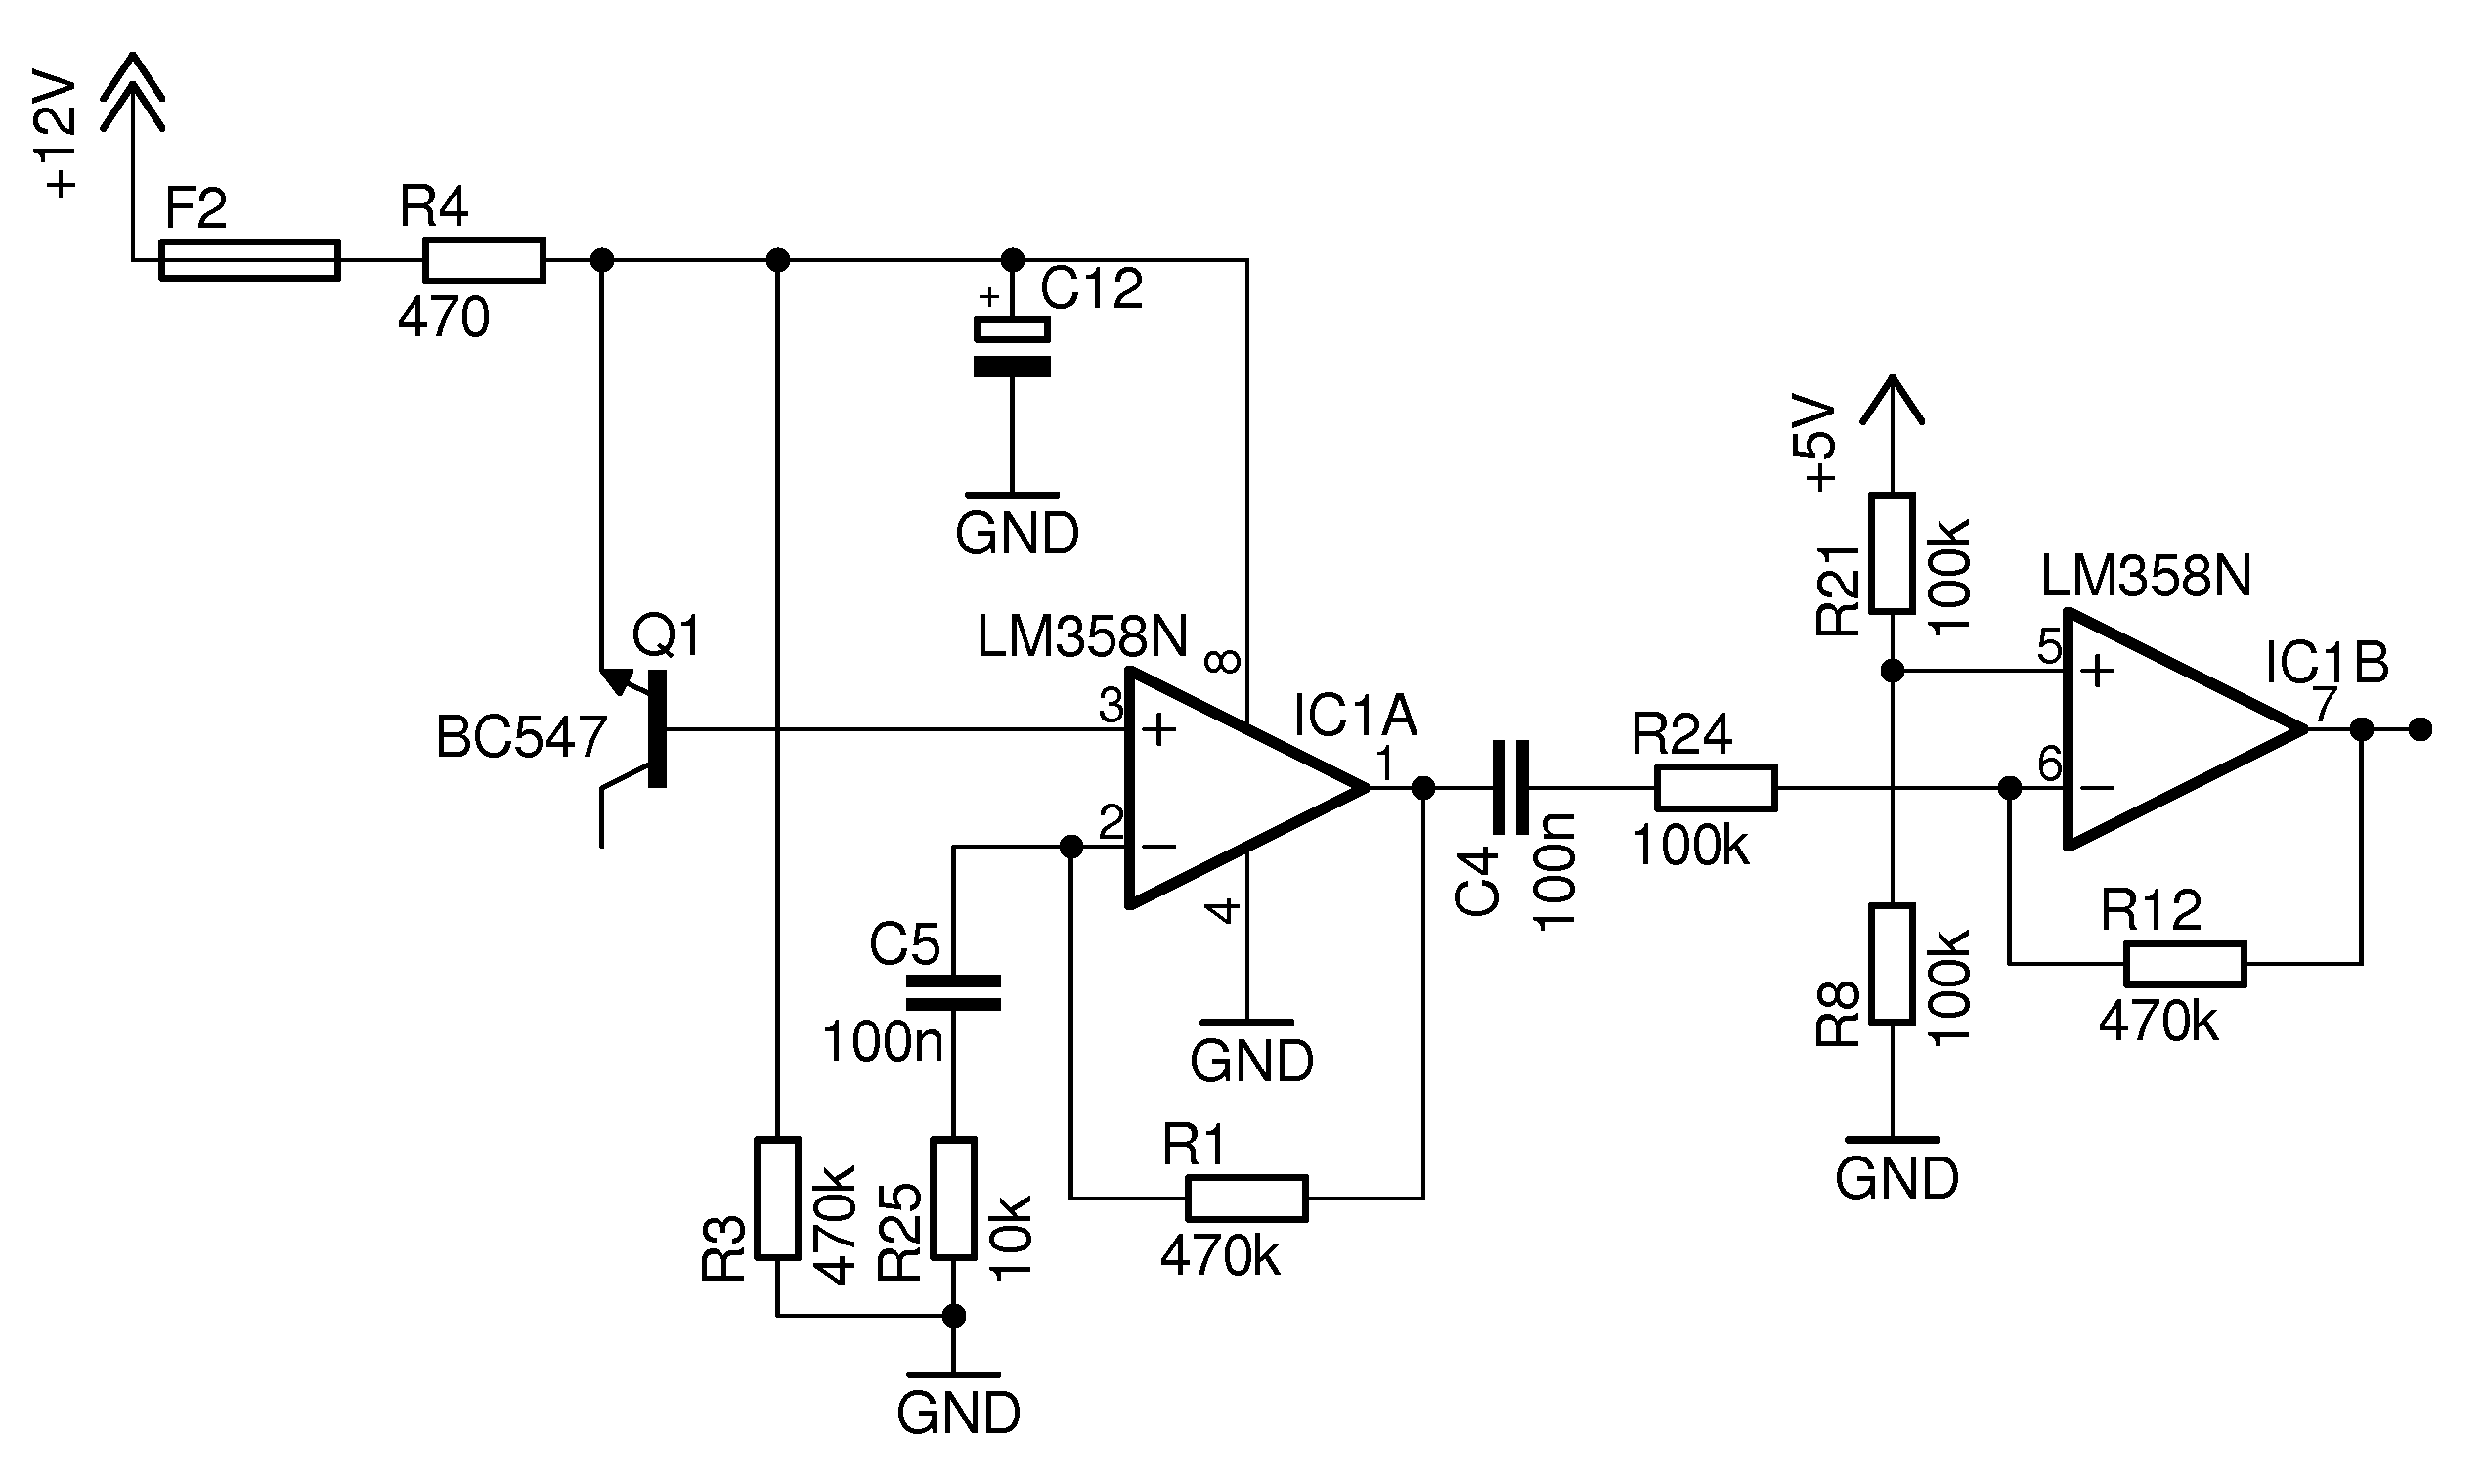
\includegraphics[scale=0.7]{hwrnd_schem}, {schematic of the hardware random generator}]
This circuit utilises the randomness of the transistor diode's breakthrough voltage to generate random voltages in the range from 0 to 5 volts. While this is quite random it does not need to be cryptographically secure, because the RNGs output is used only as input for the cryptographically secure PRNG. \\
\end{window}
\vspace{1cm}

%-----

\subsection{Pseudo-random number generator (PRNG)}
The PRNG is based on the SHA-256 hash function and is specified in Appendix A.
It has two main functions:
\begin{itemize}
 \item AddEntropy: this function adds data to the entropy pool, the input can be of arbitrary bit length
 \item GetRandomBlock: this function fills a 32 byte block of memory with a randomised bit string
\end{itemize}
An other function (GetRandomByte) uses a buffer and the GetRandomBlock function and returns a random byte.
The PRNG is periodically filled with entropy from the hardware RNG using the AddEntropy function.

%-----

\subsection{Secure serial port (QPort-tiny)}
QPort-tiny\cite{QPort-tiny} is a software stack which offers a secure communication channel over an insecure serial line. It therefore uses a preshared secret key to agree on a set of secret symmetric keys which are used for encryption. HMAC-SHA256 is used for session key generation and XTEA\cite{XTEA} is used in OFB and CFB mode for encryption. 
%-----

\subsection{External serial EEPROM}
The external serial EEPROM is used to keep the ticket databases and the flag-modify database and can be used for key-storage in the migration process. We use standard $I^2C$\cite{I2C} EEPROMs with 512KiBit or 1MiBit (24xx512\cite{24xx512} or 24xx1025\cite{24xx1025}) from Microchip\cite{microchip}. It is possible to extend the storage capabilities by using multiple EEPROMs. That makes it possible to have up to 4MiBit or 512KiBytes of storage space which normally allows more than 10,000 users.

All contents of the EEPROM are encrypted (except the keymigration-area). Shabea-16 is used to encrypt the content. We therefore divide the EEPROM space into 32 byte blocks which are encrypted separately. Every block is encrypted with an individual key which is the result of concatenation of the ''main-key''(\textit{eepromcrypt\_key}) and the block address. So we are protected from most attacks against mass storage encryption (ex. watermarking).

%-----

\subsection{Ticket-Database (TicketDB)}
This database is used to store a HMAC of the user's ticket, her/his permissions, and some statistics about the whole system.
The first element in the database is the header followed by the entries for the users.\\
\begin{tabular}{|l|c|p{8cm}|}\hline 
name & size & description \\ \hline
ID & 10 bytes & set to the ASCII string ''AnonAccess'' \\
majversion & 1 byte & major version; set to 1 \\
minversion & 1 byte & minor version; set to 0 \\
headersize & 1 byte & specifies the size of the header \\
stat & 10 bytes & statistics \\
reserved & 8 bytes & reserved field for future extensions and for alignment; set to 0 \\ \hline
\end{tabular} 

The statistics field has the following structure:\\
\begin{tabular}{|l|c|l|} \hline
name & size & description \\ \hline 
max\_users     & 2 bytes & maximum number of users \\
users          & 2 bytes & actually active user \\
admins         & 2 bytes & actually active admins \\
locked\_users  & 2 bytes & number of locked users \\
locked\_admins & 2 bytes & number of locked admins \\ \hline
\end{tabular} 

The following space of the \textit{TicketDB} is filled with user entries which have the following structure:\\
\begin{tabular}{|l|c|l|} \hline
name & size & description \\ \hline 
flags      &  1 byte  & the flags associated with the user \\
nickname   &  7 bytes & the nickname if the user decided to be known by name \\
ticketmac  & 32 bytes & HMAC from users ticket \\ \hline
\end{tabular} 

Where the flag field has the following structure: \\
\begin{tabular}{|l|c|l|} \hline
name & size & description \\ \hline 
exists            & 1 bit    &  indicates if this entry is used (1: in use; 0: free)\\
admin             & 1 bit & set if user has admin privileges, cleared otherwise \\
locked            & 1 bit & set if user is locked; cleared otherwise \\
notify\_lostadmin & 1 bit & set if user has to be notified about lost admin privileges \\
anonymous         & 1 bit & set if the user did not specify username to be stored \\
reserved          & 3 bit & reserved, should be set to 0\\ \hline
\end{tabular} 

%-----

\subsection{FlagModifying-Database (FLMDB)}
The flag-modifying-Database keeps entries which specify how a given user account should be modified. \\
\begin{tabular}{|l|c|p{8cm}|} \hline
name & size & description \\ \hline 
active     & 1 byte    & set to 1 if this entry is active; set to 0 otherwise \\
permanent  & 1 byte & set to 1 if this entry should not be removed if applied; set to 0 otherwise \\
last       & 1 bytes & if set to 1 this is the last entry to check; set to 0 otherwise \\ 
setflags   & 1 byte & specifies which bits have to be set in the userflags\\
clearflags & 1 byte & specifies which bits have to be cleared in the userflags\\
reserved   & 3 byte & reserved; set to 0\\
timestamp  & 8 bytes & timestamp of the creation of this entry\\
hnick      & 32 bytes & HMAC of the users pseudonym\\
\hline
\end{tabular}

%-----

\subsection{Key-Database (Key-DB)}
This database stores all the cryptographic keys used in the system.\\
\begin{tabular}{|l|c|p{8cm}|} \hline
name & size & description \\ \hline 
ticket\_key            & 256 bit & used to generate the HMAC from the ticket which is stored in \textit{TicketDB} \\
absign\_key      & 256 bit & used to generate the HMAC in the \textit{AuthBlock} \\
rid\_key         & 256 bit & used to encrypt the \textit{user pseudonym} \\
nick\_key        & 256 bit & used to generate the HMAC from the users nickname giving the \textit{user pseudonym} \\
timestamp\_key   & 256 bit & used to generate a new ticket by encrypting a 24 byte random string and a 8 byte timestamp \\
eepromcrypt\_key & 256 bit & used for encrypting the external EEPROMs content \\
\hline
\end{tabular}

